\chapter{Sprint 5}
\label{chap:sprint5}

The following section presents an overview of how we planned, worked and
completed sprint 5.

Sprint 5 started on 29th of October and ended on 11th of November, giving it a duration of 14 
days.

The chapter is divided into five parts, starting with the overall plan for the
sprint in Section \ref{sec:sprint5sprintplan}. Followed by the sprint backlog, which
enlists the tasks that have been chosen for the sprint. Section
\ref{sec:sprint5designAndImplementation}.
will focus on the work made to the GUI, the logic implemented in the application and the work done to the database and database access in the application.
The chapter ends with what have been tested and the corresponding results in
Section \ref{sec:sprint5testingAndResults} and a sprint review in Section
\ref{sec:sprint5sprintRetrospective}.

\section{Sprint Plan}
\label{sec:sprint5sprintplan}
The plan for sprint 5 was to finishing the user interface, look for and fix errors and refactor, document and comment code. At the end of this sprint we planned for a code freeze for the sourcecode, meaning no changes were to be made after this sprint. The sprint started with the usability test, and we made the rest of the sprintplan based on the feedback we got from this test.

\section{Sprint backlog}
This section contains a table with the sprint backlog, which is a smaller part of the product backlog. The goal is to implement the entire sprint backlog implemented during the sprint.

\begin{table}
	\begin{center}
		\begin{tabular}{|p{2.0cm}| p{8.0cm}| p{2.0cm}|p{2.0cm}|p{2.0cm}|}
			\hline
			\#  ID 	& Task 	& Story points 	& Estimated hours & Responsible \\
			\hline
 			1.1 & Refine distraction for CAPP & 2 & 8 & Yngve\\
 			\hline
 			1.2 & Fix medicine choice before unscheduled medication & 2 & 8 &Yngve\\
 			\hline
 			1.3 & Fix jumping images during child distraction & 1 & 4 & Yngve\\
 			\hline
 			1.4 & Fix correct heading in all pages & 1 & 4 & Eirik and Esben\\
 			\hline
 			2.1 & Bugfix new manuscript on Karotz & 1 & 4 & Yngve\\
 			\hline
 			2.2 & Bugfix Karotz after usability test: double RFID check & 1 & 4 & Yngve\\
  			\hline
 			3.1 & Delete old alarms & 2 & 8 & Eirik\\
 			\hline
 			4.1 & Make better layout for info about medication & 1 & 4 & Aleksander\\
 			\hline
 			5.1 & Write javadoc for all code & 3 & 12 & Esben, Eirik\\
 			\hline
 			5.2 & Remove unused code (imports, classes, etc) & 1 & 4 & Aleksander, Eirik and Esben \\
 			\hline
 			6.1 & Fix Wifi-related crashes in CAPP & 0.5 & 2 & Esben \\
 			\hline
 			6.2 & Fix Wifi-related crashes in GAPP & 0.5 & 2 & Esben \\
 			\hline
 			7.1 & Perform and document unit tests of all we access pages & 1 & 4 & Yngve \\
 			\hline
 			\bfseries{SUM} & & \bfseries{19} & \bfseries{76} & \\
 			\hline
 			\hline
		\end{tabular}
	\end{center}
	\caption{Backlog for sprint 5}
\end{table}

\section{Design and Implementation}
\label{sec:sprint5designAndImplementation}
Since this was the last sprint, the code had to be refactored and commented. During this sprint we made sure to delete all classes that were not in use, merge classes were possible and logical and mark all deprecated classes. This resulted in a much more understandable and readable code. 

After deleting all unused code, we wrote javadoc\cite{javadoc} for all code. Since javadoc is a common use among java developers, this will make the source code easier to read and understand, for people picking up the code in the future. 

\subsection{User Interface Layer}
\subsubsection{CAPP}
CAPP underwent minor changes to the user interface. The main menu had it's icons changed out, to give it a nicer, more colorful and thus more attractive look. 

The overview of how many stars the child has earned was given a bigger star at the top, to easily show how many stars the child has earned in total. 

\subsubsection{GAPP}
GAPP underwent very small changes in this sprint. To the section where users may view information about medication, we added pages for viewing information about specific medicines, and a link to the instructions images implemented earlier. 

\subsubsection{Karotz}
Based on the usability test, the manuscript for both Karotz and CAPP were updated. The counting action was reworked to include instructions for the child to press
the medicine in order to start the medication process. Also, whenever the user was told to hold a nanoz to the rabbit, they were previously told to hold it against the
rabbit's stomach. The detector is placed directly beneath the Karotz' nose, so the dialogue was changed to accomodate this. The final manuscript is laid out in detail in appendix \ref{apx:karotzManuscript}.

\subsection{Application Logic Layer}
The applications still had some bugs at the beginning of the sprint. During this sprint we smashed a lot of them. Mentioning some, we fixed a problem with which medicineID was sent to the database, a problem with deleting alarms was fixed and a problem with the alarm not letting the user turn off the sound was fixed. 


\subsection{Data Persistence Layer}
Changes were made to the following files for web access:
\begin{itemize}
  \item \emph{get\_log\_days\_for\_child.php:} This module would return days in the future, with the last recorded health state id. This behavior was
		changed so that the module doesn't return entries for future days. 
\end{itemize}


\section{Testing and Results}
\label{sec:sprint5testingAndResults}

\subsection{Testing}
During this sprint our main focus was on refactoring, commenting and bugfixing. This meant we did alot of different tests during this sprint. 
The sprint started with a usabilitytest, using CAPP and Karotz app to test if children could actually follow the instructions, and to see if our system behaved
the way we intended it to. We then did unit tests for all web access modules, to make sure the correct fields were returned from the database. Lastly we 
did several integration tests to ensure that the changes implemented after the usability test, and the rest of the system, worked as intended

Tables \ref{tab:unit5.1} through \ref{tab:unit5.15} describe the unit tests done in sprint 5. 

\begin{table} %UNIT 5.1: add_child
	\begin{center}
		\begin{tabular}{|p{3.0cm}|p{14.0cm}|}
			\hline
			\bf{Item} & \bf{Description}\\
			\hline
			\bf{ID} & UNIT5.1\\
			\bf{Description} & Test of the web access module \code{add\_child.php} \\
			\bf{Date} & 30.10.12\\
			\bf{Responsible} & Yngve\\
			\bf{Subject} & \code{add\_child.php} and database \\
			\bf{Precondition} & The database is up with the tables \code{MEDICAL\_PLANS}, \code{CHILDREN}and \code{HEALTH\_STATES}.\\
			\bf{Steps} & 
			    \begin{tabulenum}
			        \item Initiate a REST client (POSTMAN) with the URL \url{http://folk.ntnu.no/yngvesva/blopp/add\_child.php}.
			        \item Add the POST data
			        \begin{tabulitem}
			            \item \code{name}: testname
			            \item \code{persnum}: 10101012345
			            \item \code{states[]}: 1
			            \item \code{states[]}: 2
			        \end{tabulitem}
			        \item Observe the returned JSON data
			    \end{tabulenum}\\
		    \hline
			\bf{Results} & 
				The JSON data returned was:
\begin{lstlisting}[caption=JSON result from \code{add\_child.php}]
{
	post: {
		name: "testnavn",
		persnum: "10101012345",
		states: [
			"1",
			"2"
		]
	},
	q: "INSERT INTO `CHILDREN` (`id`, `name`, `pers_num`, `medical_plan_id`, `credits`) VALUES ('', 'testnavn', '10101012345', '0', '0')",
	medical_plan_q: "INSERT INTO `MEDICAL_PLANS` (`id`, `label`) VALUES ('', 'testnavn')",
	medical_plan_id: 0,
	child_id: 12,
	state_queries: [
		"INSERT INTO `CHILD_HEALTH_STATES` (`child_id`, `health_state_id`, `applies_now`, `default`) VALUES ('12', '1', '1''1')",
		"INSERT INTO `CHILD_HEALTH_STATES` (`child_id`, `health_state_id`, `applies_now`, `default`) VALUES ('12', '2', '0''0')"
	],
	all_state_ids: [
		"1",
		"2",
		"3"
	]
}
\end{lstlisting}
				We can see from the JSON result that a child was added successfully, and it got the ID 10.
				\\
			\hline
		\end{tabular}
	\end{center}
	\caption{Unit test 5.1, \code{add\_child.php}}
	\label{tab:unit5.1}
\end{table}

\begin{table} %UNIT 5.2: add_plan_dose
	\begin{center}
		\begin{tabular}{|p{3.0cm}|p{14.0cm}|}
			\hline
			\bf{Item} & \bf{Description}\\
			\hline
			\bf{ID} & UNIT5.2\\
			\bf{Description} & Test of the web access module \code{add\_plan\_dose.php}\\
			\bf{Date} & 01.11.12\\
			\bf{Responsible} & Yngve\\
			\bf{Subject} & \code{add\_plan\_dose.php} and the database\\
			\bf{Precondition} & The database is up with the tables \code{MEDICAL\_PLAN\_DOSES} and \code{CHILDREN}.\\
			\bf{Steps} &
			\begin{tabulenum}
				\item Initiate a REST client (POSTMAN) with the url \url{http://folk.ntnu.no/yngvesva/blopp/add\_plan\_dose.php}.
				\item Add the post data:
					\begin{tabulitem}
					  \item \code{child\_id}: 6
					  \item \code{health\_state\_id}: 1
					  \item \code{medicine\_id}: 1
					  \item \code{time}: 12:34:56
					\end{tabulitem}
				\item Observe the returned JSON data.
			\end{tabulenum}\\
			\hline
			\bf{Results} & The returned JSON data was:
\begin{lstlisting}[caption=JSON result from \code{add\_plan\_dose.php}]
{
    "sqlsuccess": true,
    "q": "INSERT INTO `MEDICAL_PLAN_DOSES` (`id`, `medical_plan_id`, `health_state_id`, `time`, `medicine_id`) SELECT '', C.medical_plan_id, '1', '12:34:56', '1' FROM `CHILDREN` AS C WHERE C.id='6'",
    "child_id": "6",
    "health_state_id": "1",
    "medicine_id": "1",
    "time": "12:34:56",
    "id": 40
}
\end{lstlisting}
				We see that a planned dose was added successfully by validating the queries and the parameter \code{sqlsuccess}, and checking the id 40.\\
			\hline
		\end{tabular}
	\end{center}
	\label{tab:unit5.2}
	\caption{Unit test 5.2, \code{add\_plan\_dose.php}}
\end{table}

\begin{table} %UNIT 5.3: dose_is_taken
	\begin{center}
		\begin{tabular}{|p{3.0cm}|p{14.0cm}|}
			\hline
			\bf{Item} & \bf{Description}\\
			\hline
			\bf{ID} & UNIT5.3, \\
			\bf{Description} & Test of the web access module \code{dose\_is\_taken.php}.\\
			\bf{Date} & 01.11.12\\
			\bf{Responsible} & Yngve\\
			\bf{Subject} & The database and \code{dose\_is\_taken.php}.\\
			\bf{Precondition} & The database is up with the table \code{DAY\_MEDICINE\_DOSES}.\\
			\bf{Steps} &
			\begin{tabulenum}
				\item Initiate a web browser with the GET url \url{http://folk.ntnu.no/yngvesva/blopp/dose\_is\_taken.php?dose\_id=40}
				\item Observe the returned JSON data.
			\end{tabulenum}\\
			\hline
			\bf{Results} & The returned JSON data was:
\begin{lstlisting}[caption=JSON result from \code{dose\_is\_taken.php}]
{
	sqlsuccess: true,
	dose_id: "40",
	day_date: "2012-11-01",
	query: "SELECT `id` FROM `DAY_MEDICINE_DOSES` WHERE `medical_plan_dose_id`='40' AND `day_date`='2012-11-01' LIMIT 0,1",
	result: false
}
\end{lstlisting}
			We see from the result that the dose with id 40 (added in UNIT5.2, table 
			\ref{tab:unit5.2}) has not been taken on the actual date, and by the query
			and the \code{sqlsuccess} parameter, we see that the GET module works.\\
			\hline
		\end{tabular}
	\end{center}
	\caption{Unit test 5.3, \code{dose\_is\_taken.php}}
	\label{tab:unit5.3}
\end{table}

\begin{table} %UNIT 5.4: get_available_child_states
	\begin{center}
		\begin{tabular}{|p{3.0cm}|p{14.0cm}|}
			\hline
			\bf{Item} & \bf{Description}\\
			\hline
			\bf{ID} & UNIT5.4\\
			\bf{Description} & Test of the web access module \code{get\_available\_child\_states.php}.\\
			\bf{Date} & 01.11.12\\
			\bf{Responsible} & Yngve\\
			\bf{Subject} & The database and \code{get\_available\_child\_states.php}.\\
			\bf{Precondition} & A working database with the tables \code{HEALTH\_STATES} and \code{CHILD\_HEALTH\_STATES}.\\
			\bf{Steps} &
			\begin{tabulenum}
				\item Initiate a web browser with the GET url \url{http://folk.ntnu.no/yngvesva/blopp/get\_available\_child\_states.php?child\_id=6}.
				\item Observe the returned JSON data.
			\end{tabulenum}\\
			\hline
			\bf{Results} & The returned JSON data was:
\begin{lstlisting}[caption=JSON result from \code{get\_available\_child\_states.php}]
{
	sqlsuccess: true,
	child_id: "6",
	query: "SELECT id, label FROM `HEALTH_STATES` HS WHERE HS.id IN (SELECT health_state_id FROM `CHILD_HEALTH_STATES` CHS WHERE CHS.child_id=6) LIMIT 0,10",
	rows: [
		{
			id: "1",
			label: "GREEN"
		},
		{
			id: "2",
			label: "YELLOW"
		},
		{
			id: "3",
			label: "RED"
		}
	]
}
\end{lstlisting}
			We see from the returned data that the child with $ID=6$ can have all states (\code{GREEN}, 
			\code{YELLOW} and \code{RED}), and that the module works by checking \code{sqlsuccess} and \code{query}.\\
			\hline
		\end{tabular}
	\end{center}
	\caption{Unit test 5.4, \code{get\_available\_child\_states.php}}
	\label{tab:unit5.4}
\end{table}

\begin{table} %UNIT 5.5: get_child
	\begin{center}
		\begin{tabular}{|p{3.0cm}|p{14.0cm}|}
			\hline
			\bf{Item} & \bf{Description}\\
			\hline
			\bf{ID} & UNIT5.5\\
			\bf{Description} & Test of the web access module \code{get\_child.php}.\\
			\bf{Date} & 01.11.12\\
			\bf{Responsible} & Yngve\\
			\bf{Subject} & The database and \code{get\_child.php}.\\
			\bf{Precondition} & A working database with the table \code{CHILDREN}.\\
			\bf{Steps} &
			\begin{tabulenum}
				\item Initiate a web browser with the GET url \url{http://folk.ntnu.no/yngvesva/blopp/get\_child.php?child\_id=6}.
				\item Observe the returned JSON data.
			\end{tabulenum}\\
			\hline
			\bf{Results} &
			The returned JSON data was:
\begin{lstlisting}[caption=JSON result from \code{get\_child.php}]
{
	sqlsuccess: true,
	child_id: "6",
	query: "SELECT * FROM `CHILDREN` WHERE id=6 LIMIT 0,1",
	information: {
		id: "6",
		name: "Hermann",
		pers_num: "1010354322",
		medical_plan_id: "5",
		avatar_id: "7",
		credits: "45",
		location_latitude: "0",
		location_longitude: "0"
	}
}
\end{lstlisting}
			We see from the returned data that the child with $ID=6$ is named Hermann, some other information, and that the query works.
			\\
			\hline
		\end{tabular}
	\end{center}
	\caption{Unit test 5.5, \code{get\_child.php}}
	\label{tab:unit5.5}
\end{table}

\begin{table} %UNIT 5.6: get_child_state
	\begin{center}
		\begin{tabular}{|p{3.0cm}|p{14.0cm}|}
			\hline
			\bf{Item} & \bf{Description}\\
			\hline
			\bf{ID} & UNIT5.6\\
			\bf{Description} & Test of the web access module \code{get\_child\_state.php}\\
			\bf{Date} & 01.11.12\\
			\bf{Responsible} & Yngve\\
			\bf{Subject} & The database and \code{get\_child\_state.php}.\\
			\bf{Precondition} & A working database with the tables \code{HEALTH\_STATES} and \code{CHILD\_HEALTH\_STATES}\\
			\bf{Steps} &
			\begin{tabulenum}
				\item Initiate a web browser with the GET url \url{http://folk.ntnu.no/yngvesva/blopp/get\_child\_state.php?child\_id=6}.
				\item Observe the returned JSON data.
			\end{tabulenum}\\
			\hline
			\bf{Results} & The returned JSON data was:
\begin{lstlisting}[caption=Returned JSON data from \code{get\_child\_state.php}]
{
	sqlsuccess: true,
	child_id: "6",
	query: "SELECT id, label FROM `HEALTH_STATES` HS WHERE HS.id IN (SELECT health_state_id FROM `CHILD_HEALTH_STATES` CHS WHERE CHS.child_id=6 AND CHS.applies_now=1) LIMIT 0,1",
	state: {
		id: "1",
		label: "GREEN"
	}
}
\end{lstlisting}
			We see from the returned data that the child with $ID=6$ is in the green state, and that the module works.\\
			\hline
		\end{tabular}
	\end{center}
	\caption{Unit test 5.6, \code{get\_child\_state.php}}
	\label{tab:unit5.6}
\end{table}

\begin{table} %UNIT 5.7: get_doses_for_current_state
	\begin{center}
		\begin{tabular}{|p{3.0cm}|p{14.0cm}|}
			\hline
			\bf{Item} & \bf{Description}\\
			\hline
			\bf{ID} & UNIT5.7\\
			\bf{Description} & Test of the web access module \code{get\_doses\_for\_current\_state.php}.\\
			\bf{Date} & 01.11.12\\
			\bf{Responsible} & Yngve\\
			\bf{Subject} & The database and \code{get\_doses\_for\_current\_state.php}\\
			\bf{Precondition} & A working database with the tables \code{MEDICAL\_PLAN\_DOSES}, \code{DAY\_MEDICINE\_DOSES} and \code{CHILD\_HEALTH\_STATES}.\\
			\bf{Steps} &
			\begin{tabulenum}
				\item Initiate a web browser with the GET url \url{http://folk.ntnu.no/yngvesva/blopp/get\_doses\_for\_current\_state.php?child\_id=6}.
				\item Observe the returned JSON data.
			\end{tabulenum}\\
			\hline
			\bf{Results} & The returned JSON data was:
\begin{lstlisting}[caption=Returned JSON data for \code{get\_doses\_for\_current\_state.php}]
{
	sqlsuccess: true,
	child_id: "6",
	query: "SELECT Mpd.id, Mpd.medical_plan_id, Mpd.health_state_id, Mpd.time, Mpd.medicine_id, M.color AS 'medicine_color', M.name AS 'medicine_name' FROM `MEDICAL_PLAN_DOSES` AS Mpd, `MEDICINES` AS M WHERE Mpd.medical_plan_id IN (SELECT C.medical_plan_id FROM `CHILDREN` AS C WHERE C.id=6) AND Mpd.id NOT IN (SELECT DMD.medical_plan_dose_id FROM `DAY_MEDICINE_DOSES` AS DMD WHERE DMD.medical_plan_dose_id=Mpd.id AND DMD.day_date='2012-11-04') AND Mpd.medicine_id = M.id AND Mpd.health_state_id IN (SELECT HS.health_state_id FROM `CHILD_HEALTH_STATES` AS HS WHERE HS.child_id=6 AND HS.applies_now='1') LIMIT 0,100",
	rows: [
		{
			id: "41",
			medical_plan_id: "5",
			health_state_id: "1",
			time: "01:09:00",
			medicine_id: "1",
			medicine_color: "BLUE",
			medicine_name: "Flutide"
		}
	]
}
\end{lstlisting}
			From the returned data we see that the child with $ID=6$ has yet to take Flutide today, which 
			should be taken at 01:09:00. We can also validate the SQL query, and see that $sqlsuccess=true$,
			which means that the module works.\\
			\hline
		\end{tabular}
	\end{center}
	\caption{Unit test 5.7, \code{get\_doses\_for\_current\_state.php}}
	\label{tab:unit5.7}
\end{table}

\begin{table} %UNIT 5.8: get_instructions
	\begin{center}
		\begin{tabular}{|p{3.0cm}|p{14.0cm}|}
			\hline
			\bf{Item} & \bf{Description}\\
			\hline
			\bf{ID} & UNIT5.8\\
			\bf{Description} & Test of the web access module \code{get\_instructions.php}.\\
			\bf{Date} & 01.11.12\\
			\bf{Responsible} & Yngve\\
			\bf{Subject} & The database and \code{get\_instructions.php}.\\
			\bf{Precondition} & A working database with the table \code{MEDICINE\_INSTRUCTIONS}.\\
			\bf{Steps} &
			\begin{tabulenum}
				\item Initialize a web browser with the GET url \url{http://folk.ntnu.no/yngvesva/blopp/get\_instructions.php?medicine\_id=1}.
				\item Observe the returned JSON data.
			\end{tabulenum}\\
			\hline
			\bf{Results} & The returned JSON data was: 
\begin{lstlisting}[caption=Returned JSON from \code{get\_instructions.php}]
{
	sqlsuccess: true,
	child_id: "1",
	query: "SELECT * FROM `MEDICINE_INSTRUCTIONS` WHERE id IN (SELECT instructions_id FROM `MEDICINES` WHERE `id`='1') LIMIT 0,1",
	instructions: {
		id: "1",
		url: "medicine_flutide_50microg.jpg",
		information: "Et inhalasjonssteroid som brukes fast slik legen har bestemt. Effekten ses forst etter noen dagers bruk, og gjor at betennelsesreaksjonen i lungene til barnet demper seg. Dette hindrer barnets astma/betennelsesreaksjon i a utvikle seg og hindrer utvikling av sykdommen.",
		effect: "Alle sprayinhalasjoner ma gis pa inhalasjonskammer (Aerochamber, Optichamber, Babyhaler eller lignende) for a sikre at barnet far pustet inn medisinen pa riktig mate. Etter inhalasjon med steroider ma barnet alltid skylle munn, drikke eller pusse tenner for a fjerne rester av pulver fra munnen. Blir restene igjen i munnen kan det oppsta en smertefull soppinfeksjon i munnen."
	}
}
\end{lstlisting}
			We see from the JSON data that the module works by checking the query 
			and the variable \code{sqlsuccess}. We get the information that the medicine 
			with $ID=1$ has three types of instructions: an image given by an URI, 
			a general information field and a field to explain the effects.\\
			\hline
		\end{tabular}
	\end{center}
	\caption{Unit test 5.8, \code{get\_instructions.php}}
	\label{tab:unit5.8}
\end{table}

\begin{table} %UNIT 5.9: get_log_days_for_child
	\begin{center}
		\begin{tabular}{|p{3.0cm}|p{14.1cm}|}
			\hline
			\bf{Item} & \bf{Description}\\
			\hline
			\bf{ID} & UNIT5.9\\
			\bf{Description} & Test of the web access module \code{get\_log\_days\_for\_child.php}.\\
			\bf{Date} & 03.11.12\\
			\bf{Responsible} & Yngve\\
			\bf{Subject} & The database and \code{get\_log\_days\_for\_child.php}\\
			\bf{Precondition} & A working database with the tables \code{DAY\_MEDICINE\_DOSES} and \code{CHILDREN\_LOG\_DAYS}.\\
			\bf{Steps} &
			\begin{tabulenum}
				\item Initialize a web browser with the GET url \url{http://folk.ntnu.no/yngvesva/blopp/get\_log\_days\_for\_child.php?child\_id=6}
				\item Observe the resulting JSON data.
			\end{tabulenum}\\
			\hline
			\bf{Results} & The returned JSON data was:
\begin{lstlisting}[caption=Returned JSON data for \code{get\_log\_days\_for\_child.php}]
{
    sqlsuccess: true,
    child_id: "6",
    year: "2012",
    month: "11",
    query: "SELECT * FROM `DAY_MEDICINE_DOSES` WHERE `child_id`='6' AND YEAR(`day_date`)='2012' AND MONTH(`day_date`)='11' LIMIT 0,100",
    statuses_query: "SELECT `date`, `child_id`, `health_state_id` FROM `CHILDREN_LOG_DAYS` WHERE `child_id`='6' ORDER BY `date` ASC",
    days: [{
        date: "2012-11-01",
        health_state_id: "1",
        doses: []
    }, {
        date: "2012-11-02",
        health_state_id: "1",
        doses: [{
            id: "126",
            reward: "1",
            time: "00:00:01",
            day_date: "2012-11-02",
            child_id: "6",
            medicine_id: "1",
            health_state_id: "1",
            medical_plan_dose_id: "0",
            pollen_state_id: "0"
        }]
    }, {
        date: "2012-11-03",
        health_state_id: "3",
        doses: []
    }]
}
\end{lstlisting}
			As we see from the returned data, the child with $ID=6$ has one registered dose 
			in november, and the date was the third. We also see that the health state was
			changed to $health\_state\_id=3$ on the third. It is clear that the module is
			working because of the returned data, validating the queries and the variable
			\code{sqlsuccess}. 
			\\
			\hline
		\end{tabular}
	\end{center}
	\caption{Unit test 5.9, \code{get\_log\_days\_for\_child.php}}
	\label{tab:unit5.9}
\end{table}

\begin{table} %UNIT 5.10: get_log_for_child
	\begin{center}
		\begin{tabular}{|p{3.0cm}|p{14.0cm}|}
			\hline
			\bf{Item} & \bf{Description}\\
			\hline
			\bf{ID} & UNIT5.10\\
			\bf{Description} & Test of the web access module \code{get\_log\_for\_child.php}.\\
			\bf{Date} & 03.11.12\\
			\bf{Responsible} & Yngve\\
			\bf{Subject} & The database and \code{get\_log\_for\_child.php}.\\
			\bf{Precondition} & A working database with the table \code{DAY\_MEDICINE\_DOSES}.\\
			\bf{Steps} &
			\begin{tabulenum}
				\item Initialize a web browser with the GET url \url{http://folk.ntnu.no/yngvesva/blopp/get\_log\_for\_child.php?child\_id=6}.
				\item Observe the returned JSON data.
			\end{tabulenum}\\
			\hline
			\bf{Results} & The resulting JSON data was:
\begin{lstlisting}[caption=Returned JSON data from \code{get\_log\_for\_child.php}]
{
    sqlsuccess: true,
    child_id: "6",
    year: "2012",
    month: "11",
    query: "SELECT * FROM `DAY_MEDICINE_DOSES` WHERE `child_id`=6 AND YEAR(`day_date`)=2012 AND MONTH(`day_date`)=11 LIMIT 0,100",
    days: [
        {
            id: "126",
            reward: "1",
            time: "00:00:01",
            day_date: "2012-11-02",
            child_id: "6",
            medicine_id: "1",
            health_state_id: "1",
            medical_plan_dose_id: "0",
            pollen_state_id: "0"
        }
    ]
}
\end{lstlisting}
			We see from the returned data that there was one logged medication
			and that the module works from checking the query and the variable
			\code{sqlsuccess}.
			\\
			\hline
		\end{tabular}
	\end{center}
	\caption{Unit test 5.10, \code{get\_log\_for\_child.php}}
	\label{tab:unit5.10}
\end{table}

\begin{table} %UNIT 5.11: get_plan
	\begin{center}
		\begin{tabular}{|p{3.0cm}|p{14.0cm}|}
			\hline
			\bf{Item} & \bf{Description}\\
			\hline
			\bf{ID} & UNIT5.11\\
			\bf{Description} & Test of the web access module \code{get\_plan.php}.\\
			\bf{Date} & 04.11.12\\
			\bf{Responsible} & Yngve\\
			\bf{Subject} & The database and \code{get\_plan.php}.\\
			\bf{Precondition} & A working database with the tables \code{MEDICAL\_PLAN\_DOSES} and \code{CHILDREN}.\\
			\bf{Steps} &
			\begin{tabulenum}
				\item Initialize a web browser with the GET url \url{http://folk.ntnu.no/yngvesva/blopp/get\_plan.php?child\_id=6}.
				\item Observe the returned JSON data.
			\end{tabulenum}\\
			\hline
			\bf{Results} & The returned JSON data was:
\begin{lstlisting}[caption=Returned JSON data for \code{get\_plan.php}]
{
	sqlsuccess: true,
	child_id: "6",
	query: "SELECT Mpd.id, Mpd.medical_plan_id, Mpd.health_state_id, Mpd.time, Mpd.medicine_id, M.color AS 'medicine_color', M.name AS 'medicine_name' FROM `MEDICAL_PLAN_DOSES` AS Mpd, `MEDICINES` AS M WHERE Mpd.medical_plan_id IN (SELECT medical_plan_id FROM `CHILDREN` C WHERE C.id=6) AND Mpd.medicine_id = M.id LIMIT 0,100",
	rows: [
		{
			id: "41",
			medical_plan_id: "5",
			health_state_id: "1",
			time: "01:09:00",
			medicine_id: "1",
			medicine_color: "BLUE",
			medicine_name: "Flutide"
		}
	]
}
\end{lstlisting}
			We see from the returned data that there is one medication of
			Flutide planned at 01:09:00. We conclude that the module is
			working from looking at the query and checking the variable
			\code{sqlsuccess}.
			\\
			\hline
		\end{tabular}
	\end{center}
	\caption{Unit test 5.11, $get\_plan.php$}
	\label{tab:unit5.11}
\end{table}

\begin{table} %UNIT 5.12: register_medicine_taken
	\begin{center}
		\begin{tabular}{|p{3.0cm}|p{14.0cm}|}
			\hline
			\bf{Item} & \bf{Description}\\
			\hline
			\bf{ID} & UNIT5.12\\
			\bf{Description} & Test of the web access module \code{register\_medicine\_taken.php}.\\
			\bf{Date} & 04.11.12\\
			\bf{Responsible} & Yngve\\
			\bf{Subject} & The database and \code{register\_medicine\_taken.php}.\\
			\bf{Precondition} & A working database with the tables \code{DAY\_MEDICINE\_DOSES}, \code{HEALTH\_STATES} and \code{CHILDREN}.\\
			\bf{Steps} &
			\begin{tabulenum}
				\item Initialize a REST client with the URL \url{http://folk.ntnu.no/yngvesva/blopp/register\_medicine\_taken.php}.
				\item Add the POST parameters:
					\begin{tabulitem}
					  \item \code{child\_id}: 6
					  \item \code{medicine\_id}: 1
					  \item \code{day\_date}: 2012-09-03
					  \item \code{health\_state\_id}: 2
					\end{tabulitem}
				\item Observe the returned JSON data.
			\end{tabulenum}\\
			\hline
			\bf{Results} & The returned JSON data was:
\begin{lstlisting}[caption=Returned JSON data from \code{register\_medicine\_taken.php}]
{
    "sqlsuccess": true,
    "post": {
        "child_id": "6",
        "medicine_id": "1",
        "day_date": "2012-09-30",
        "health_state_id": "2"
    },
    "q": "INSERT INTO `DAY_MEDICINE_DOSES` (`id`, `reward`, `time`, `day_date`, `child_id`, `medicine_id`, `health_state_id`, `medical_plan_dose_id`, `pollen_state_id`) VALUES ('', '2', '00:00:01', '2012-09-30', '6', '1', '2', '', '')",
    "reward": "2",
    "unique": true
}
\end{lstlisting}
			We see from the returned data, by looking at \code{query} and \code{sqlsuccess},
			that an entry was added to the log. It was given a default time of
			00:00:01 since we did not specify it, and the returned calculated
			reward was 2. We can conclude that the dose was registered
			successfully and the module works.
			\\
			\hline
		\end{tabular}
	\end{center}
	\caption{Unit test 5.12, \code{register\_medicine\_taken.php}}
	\label{tab:unit5.12}
\end{table}

\begin{table} %UNIT 5.13: remove\_plan\_dose.php
	\begin{center}
		\begin{tabular}{|p{3.0cm}|p{14.0cm}|}
			\hline
			\bf{Item} & \bf{Description}\\
			\hline
			\bf{ID} & UNIT5.13\\
			\bf{Description} & Test of the web access module \code{remove\_plan\_dose.php}.\\
			\bf{Date} & 04.11.12\\
			\bf{Responsible} & Yngve\\
			\bf{Subject} & The database and \code{remove\_plan\_dose.php}.\\
			\bf{Precondition} & A working database with the table \code{MEDICAL\_PLAN\_DOSES}.\\
			\bf{Steps} &
			\begin{tabulenum}
				\item Initialize a REST client (POSTMAN) with the URL \url{http://folk.ntnu.no/yngvesva/blopp/remove\_plan\_dose.php}.
				\item Add the POST parameter:
					\begin{tabulitem}
					  \item $id$: 41
					\end{tabulitem}
				\item Observe the returned JSON data.
			\end{tabulenum}\\
			\hline
			\bf{Results} & The returned JSON data was:
\begin{lstlisting}[caption=Returned JSON data from \code{remove\_plan\_dose.php}]
{
    "sqlsuccess": true,
    "q": "DELETE FROM `MEDICAL_PLAN_DOSES` WHERE id='41'",
    "id": "41",
    "num_deleted": 1
}
\end{lstlisting}
			We conclude from the query, \code{sqlsuccess} and \code{num\_deleted} that
			the row with $ID=41$ was deleted and that the module works.
			\\
			\hline
		\end{tabular}
	\end{center}
	\caption{Unit test 5.13, \code{remove\_plan\_dose.php}}
	\label{tab:unit5.13}
\end{table}

\begin{table} %UNIT 5.14: remove_plan_medicine_at_time
	\begin{center}
		\begin{tabular}{|p{3.0cm}|p{14.0cm}|}
			\hline
			\bf{Item} & \bf{Description}\\
			\hline
			\bf{ID} & UNIT5.14\\
			\bf{Description} & Test of the web access module \code{remove\_plan\_medicine\_at\_time.php}.\\
			\bf{Date} & 04.11.12\\
			\bf{Responsible} & Yngve\\
			\bf{Subject} & The database and \code{remove\_plan\_medicine\_at\_time.php}\\
			\bf{Precondition} & A working database \\
			\bf{Steps} &
			\begin{tabulenum}
				\item Initiate a REST client (POSTMAN) with the URL \url{http://folk.ntnu.no/yngvesva/blopp/remove\_plan\_medicine\_at\_time.php}.
				\item Add the POST parameters:
					\begin{tabulitem}
					  \item \code{time}: 12:34:56
					  \item \code{medicine\_id}: 1
					  \item \code{child\_id}: 6
					  \item \code{health\_state\_id}: 3
					\end{tabulitem}
				\item Observe the returned JSON data.
			\end{tabulenum}\\
			\hline
			\bf{Results} & The returned data is:
\begin{lstlisting}[caption=Returned JSON data from \code{remove\_plan\_medicine\_at\_time.php}]
{
    "sqlsuccess": true,
    "q": "INSERT INTO `MEDICAL_PLAN_DOSES` (`id`, `medical_plan_id`, `health_state_id`, `time`, `medicine_id`) SELECT '', C.medical_plan_id, '3', '12:34:56', '1' FROM `CHILDREN` AS C WHERE C.id='6'",
    "child_id": "6",
    "health_state_id": "3",
    "medicine_id": "1",
    "time": "12:34:56",
    "id": 44
}
\end{lstlisting}
			We see from the data that a medication dose was removed, and
			by the query and \code{sqlsuccess} we see that the module works.
			\\
			\hline
		\end{tabular}
	\end{center}
	\caption{Unit test 5.14, \code{remove\_plan\_medicine\_at\_time.php}}
	\label{tab:unit5.14}
\end{table}

\begin{table} %UNIT 5.15, set_child_state
	\begin{center}
		\begin{tabular}{|p{3.0cm}|p{14.0cm}|}
			\hline
			\bf{Item} & \bf{Description}\\
			\hline
			\bf{ID} & UNIT5.15\\
			\bf{Description} & Test of the web access module \code{set\_child\_state.php}.\\
			\bf{Date} & 05.11.12\\
			\bf{Responsible} & Yngve\\
			\bf{Subject} & The database and \code{set\_child\_state.php}.\\
			\bf{Precondition} & A working database with the tables \code{CHILD\_HEALTH\_STATES} and \code{CHILDREN\_LOG\_DAYS}.\\
			\bf{Steps} &
			\begin{tabulenum}
				\item Initialize a REST client (POSTMAN) with the URL \url{http://folk.ntnu.no/yngvesva/bopp/set\_child\_state.php}.
				\item Add the POST parameters:
					\begin{tabulitem}
					  \item \code{child\_id}: 6
					  \item \code{state\_id}: 2
					\end{tabulitem}
				\item Observe the returned JSON data.
			\end{tabulenum}\\
			\hline
			\bf{Results} & The returned JSON data was:
\begin{lstlisting}[caption=Returned JSON from \code{set\_child\_state.php}]
{
    "sqlsuccess": true,
    "child_id": "6",
    "state_id": "2",
    "update_query": "UPDATE `CHILD_HEALTH_STATES` SET applies_now = IF(health_state_id = '2', 1, 0) WHERE child_id='6'",
    "insert_query": "REPLACE INTO `CHILDREN_LOG_DAYS` (`date`, `child_id`, `pollen_state_id`, `health_state_id`)  VALUES ('2012-11-05', '6', '1', '2')"
}
\end{lstlisting}
			We see from the returned JSON data that two tables were updated: the child's current
			state, and the log of state changes. We conclude that the module works because of
			the queries and the variable \code{sqlsuccess}.
			\\
			\hline
		\end{tabular}
	\end{center}
	\caption{Unit test 5.15, \code{set\_child\_state.php}}
	\label{tab:unit5.15}
\end{table}

%\begin{table}
%	\begin{center}
%		\begin{tabular}{|p{3.0cm}|p{14.0cm}|}
%			\hline
%			\bf{Item} & \bf{Description}\\
%			\hline
%			\bf{ID} & \\
%			\bf{Description} & \\
%			\bf{Date} & \\
%			\bf{Responsible} & \\
%			\bf{Subject} & \\
%			\bf{Precondition} & \\
%			\bf{Steps} &
%			\begin{tabulenum}
%				\item ~
%			\end{tabulenum}\\
%			\hline
%			\bf{Results} & \\
%			\hline
%		\end{tabular}
%	\end{center}
%	\caption{Unit test X.Y, Z}
%	\label{tab:unitX.Y}
%\end{table}

\begin{table}
	\begin{center}
		\begin{tabular}{|p{3.0cm}|p{14.0cm}|}
			\hline
			\bf{Item} & \bf{Description}\\
			\hline
			\bf{ID} & USABILITY5.1\\
			\bf{Description} & Test to see if the children can follow the isntructions given and take their medicine correctly when an alarm is given.\\
			\bf{Date} & 30.10.2012\\
			\bf{Responsible} & Eirik\\
			\bf{Subject} & The Karotz application and CAPP\\
			\bf{Precondition} & 
				\begin{tabulitem}
					\item Working version of CAPP and the karotz application.
					\item The child registered in the database is in the correct health state.
					\item Child and one parent present. The parent should be familiar with giving asthma medications.
					\item Wireless wpa2 secured connection.
				\end{tabulitem}\\
			\bf{Steps} &
			\begin{tabulenum}
				\item Explain the test for the children, in an easy to understand way.
				\item Set up an alarm to go off.
				\item Let the parent get the alarm, and see how well the child and parent is able to follow the instructions given by the system.
			\end{tabulenum}\\
			\hline
			\bf{Results} & Generally the system worked as intended. The children successfully took their medicine, and had little trouble following the instructions.
							We discovered some errors relating to the alarm, aswell as some of the distraction sequence bugging, some parts skipped stages if the child
							pressed more than once, others had inaccurate instructions (like holding the Nanoz infront of karotz belly, when it's the nose it needs to be
							in front of).\\
			\hline
		\end{tabular}
	\end{center}
	\caption{USABILITY5.1}
	\label{tab:usability5.1}
\end{table}

\begin{table}
	\begin{center}
		\begin{tabular}{|p{3.0cm}|p{14.0cm}|}
			\hline
			\bf{Item} & \bf{Description}\\
			\hline
			\bf{ID} & INTEGRATION5.1\\
			\bf{Description} & Test of CAPPs alarm and distraction sequences.\\
			\bf{Date} & 06.11.12\\
			\bf{Responsible} & Eirik\\
			\bf{Subject} & CAPP\\
			\bf{Precondition} & 
				\begin{tabulitem}
					\item Working version of CAPP installed on phone or AVD (Android Virtual Device).
					\item Internetconnection for databaseaccess.
					\item Medicationplans for the correct healthstate registered in the database.
				\end{tabulitem}\\
			\bf{Steps} &
			\begin{tabulenum}
				\item Turn on the phone or AVD, and wait until the time of the alarm.
				\item Receive the alarm.
				\item Press the medicine to start the distraction sequence
				\item Follow the instructions and take note if any instructions are skipped or missing.
			\end{tabulenum}\\
			\hline
			\bf{Results} & We found that the alarm set alarms for all healthstates, not just the one the child was currently in. Aside from this, the alarm fired correctly.
						Some of the changes we had done after the usability test made one of the sound files and animations in the distraction sequence 
						unsynchronized. Since the distractionsequence have checkpoints where the user have to interact with the application, only that 
						specific part of the distraction was out of synch, the rest ran as intended.\\
			\hline
		\end{tabular}
	\end{center}
	\caption{INTEGRATION5.1}
	\label{tab:integration5.1}
\end{table}

\begin{table}
	\begin{center}
		\begin{tabular}{|p{3.0cm}|p{14.0cm}|}
			\hline
			\bf{Item} & \bf{Description}\\
			\hline
			\bf{ID} & INTEGRATION5.2\\
			\bf{Description} & Testing that the log updates correctly based on registered medication and pollen feed.\\
			\bf{Date} & 06.11.12\\
			\bf{Responsible} & Esben\\
			\bf{Subject} & GAPP\\
			\bf{Precondition} & 
				\begin{tabulitem}
					\item Working version of GAPP installed on phone or AVD.
					\item Internetconnection for databaseaccess.
					\item Completed medications and pollen feeds registered in the database.
				\end{tabulitem}\\
			\bf{Steps} &
			\begin{tabulenum}
				\item Open GAPP on the phone or AVD.
				\item Navigate to the log.
				\item Check if the visual representation in the log corresponds to the data in the database.
			\end{tabulenum}\\
			\hline
			\bf{Results} & The log updated correctly.\\
			\hline
		\end{tabular}
	\end{center}
	\caption{INTEGRATION5.2}
	\label{tab:integration5.2}
\end{table}

\clearpage{}
\begin{table}
	\centering
		\begin{tabular}{|p{3.0cm}|p{14.0cm}|}
			\hline
			\bf{Item} & \bf{Description}\\
			\hline
			\bf{ID} & INTEGRATION5.3\\
			\bf{Description} & Testing that the medicationplans is correctly registered to their respective healthstates\\
			\bf{Date} & 05.11.12\\
			\bf{Responsible} & Eirik\\
			\bf{Subject} & GAPP\\
			\bf{Precondition} & 
				\begin{tabulitem}
					\item Working version of GAPP installed on phone or AVD.
					\item Internetconnection for databaseaccess.
					\item Medicationplans registered to various healthstates.
				\end{tabulitem}\\
			\bf{Steps} &
			\begin{tabulenum}
				\item Open GAPP on the phone or AVD.
				\item Navigate to medisinplan page.
				\item Choose each of the healthstates in turn, and see if the medicines listed under each corresponds to the medicationplans in the database.
			\end{tabulenum}\\
			\hline
			\bf{Results} & The medicationplans is correctly registered to their respective healthstates.\\
			\hline
		\end{tabular}
	\caption{INTEGRATION5.3}
	\label{tab:integration5.3}
\end{table}

% \begin{table}
% 	\begin{center}
% 		\begin{tabular}{|p{3.0cm}|p{14.0cm}|}
% 			\hline
% 			\bf{Item} & \bf{Description}\\
% 			\hline
% 			\bf{ID} & \\
% 			\bf{Description} & \\
% 			\bf{Date} & \\
% 			\bf{Responsible} & \\
% 			\bf{Subject} & \\
% 			\bf{Precondition} & \\
% 			\bf{Steps} &
% 			\begin{enumerate}
% 				\item ~
% 			\end{enumerate}\\
% 			\hline
% 			\bf{Results} & \\
% 			\hline
% 		\end{tabular}
% 	\end{center}
% 	\caption{Unit test template}
% \end{table}

\subsection{Results}
The usability test gave us much feedback on the system, and several errors that had to be fixed. The complete testresults can be found in section \ref{sec:usabilitytestonchildren}, but the main issues were centered around the alarms in CAPP, and the distraction sequence being vulnerable to skipping instructions if the children pressed too fast, 
which was often the case.

The unit tests performed during this sprint all returned the expected results, which then allowed us to move on to the integration tests we had planned. These uncovered some more 
issues that either wasn't caught by the usability test, or were a result of the changes we made in response to the usability test. The new dialogue added to the CAPP distraction sequence meant that some of the animations now were not synchronized with the sound of the Karotz counting. To fix this we made separate manuscripts for the android version and the Karotz, making it easier to synchronize.
We also discovered a problem where the alarms were registered from all health states, not just the one the child is currently in, and sending many more alarms than necessary. This problem was fixed by a method checking the health state before invoking alarms. 

\section{Sprint Retrospective}
This section contains an evaluation of the sprint. The evaluation is done mainly by the us, but feedback from the customers are added to the retrospect.

\label{sec:sprint5sprintRetrospective}

\subsection{What went well?}
We finished the implementation of desired functionality in time. Even though not all functional requirements were fulfilled, the requirements fulfilled are done properly and without major errors. 

\subsection{What shall we start doing?}
\begin{enumerate}
	\item Focus only on the report and the presentation
\end{enumerate}

\subsection{What could have gone better?}
All went very well during this sprint. 

\subsection{What should we stop doing?}
The sourcecode is now under code-freeze. If errors are found, we should report them in the section for further work. 

\subsection{Sprint Burndown Chart}

\begin{figure}
	\begin{center}
		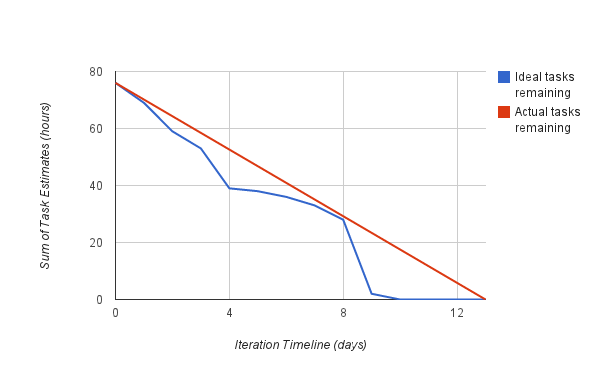
\includegraphics[width=15cm]{Pictures/Charts/Sprint5burndown}
	\end{center}
	\caption{Sprint 5 burndown chart}
	\label{fig:sprint5burndown}
\end{figure}

\begin{table}
	\begin{center}
 	\begin{sideways}
 		\begin{tabular}{| l | p{6.5cm} | c | c | l | l | l | }
 			\hline
			\#  ID 	& Task 	& Story points 	& Estimated hours & Actual & Estimated left & Responsible \\
			\hline
 			1.1 & Refine distraction for CAPP & 2 & 8 & 6 & 0 & Yngve\\
 			\hline
 			1.2 & Fix medicine choice before unscheduled medication & 2 & 8 & 7 & 0 & Yngve\\
 			\hline
 			1.3 & Fix jumping images during child distraction & 1 & 4 & 4 & 0 & Yngve\\
 			\hline
 			1.4 & Fix correct heading in all pages & 1 & 4 & 4 & 0 & Eirik and Esben\\
 			\hline
 			2.1 & Bugfix new manuscript on Karotz & 1 & 4 & 2 & 0 & Yngve\\
 			\hline
 			2.2 & Bugfix Karotz after usability test: double RFID check & 1 & 4 & 1 & 0 & Yngve\\
 			\hline
 			3.1 & Implement Thobias' changes to the report & 1 & 4 & 4 & 0 & Yngve\\
 			\hline
 			3.2 & Document usability testing, add usability test to sprint 4 & 1 & 4 & 4 & 0 & Eirik\\
 			\hline
 			4.1 & Delete old alarms & 2 & 8 & 8 & 0 & Eirik\\
 			\hline
 			5.1 & Make better layout for info about medication & 1 & 4 & 4 & 0 & Aleksander\\
 			\hline
 			6.1 & Write javadoc for all code & 3 & 12 & 7 & 0 & Esben, Eirik\\
 			\hline
 			6.2 & Remove unused code (imports, classes, etc) & 1 & 4 & 3 & 0 & Aleksander, Eirik and Esben \\
 			\hline
 			7.1 & Fix Wifi-related crashes in CAPP & 0.5 & 2 & 1 & 0 & Esben \\
 			\hline
 			7.2 & Fix Wifi-related crashes in GAPP & 0.5 & 2 & 1 & 0 & Esben \\
 			\hline
 			8.1 & Perform and document unit tests of all we access pages & 1 & 4 & 8 & 0 & Yngve \\
 			\hline
 			\bfseries{SUM} & & \bfseries{19} & \bfseries{72} & \bfseries{64} & \bfseries{0} & \\
 			\hline
 		\end{tabular}
 	\end{sideways}
 	\end{center}
 	\caption{Sprint Retrospective, Sprint 5}
 	\label{tab:sprint5burndown}
\end{table}

Table \ref{tab:sprint5burndown} and figure \ref{fig:sprint5burndown} show the burndown chart for the fifth and final sprint. Since we had
a reduced amount of story points for this sprints, everything was completed three days before schedule.

We had planned 19 story points for the fifth sprint, which meant 72 estimated work hours. We worked for a total of 64 hours, and had 0 hours
left at the end of the sprint, so all 19 story points were completed. The reduced work speed when compared to other sprints can be explained
by a shifted focus from programming tasks which are documented in the sprint, to planning and documentation exercises related to the usability
test, the report and the final presentation. These hours are not formalized as sprint tasks and are therefore not included in the estimates.
We were satisfied with the sprint result.

\subsection{Screenshots}
Since this was our last sprint, we have included some screenshots of the work that is done.


\subsection{GAPP - Screenshots}
\label{sec:gapp-screenshots}
\begin{figure}
	\begin{minipage}[b]{0.4\linewidth}
		\centering
			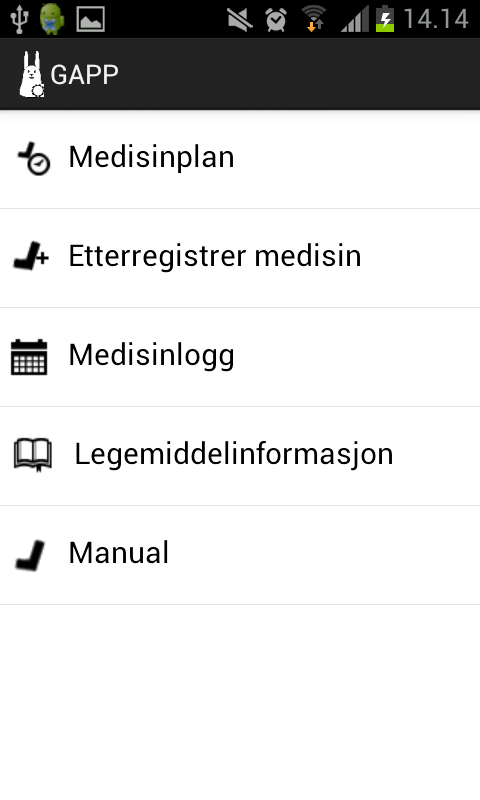
\includegraphics[width=0.20\paperwidth]{Pictures/Screenshots/gapp_main_menu.png}
		\caption{GAPP main menu}
		\label{fig:gapp-main-menu}
	\end{minipage}
	\hspace{3cm}
	\begin{minipage}[b]{0.4\linewidth}
		\centering
		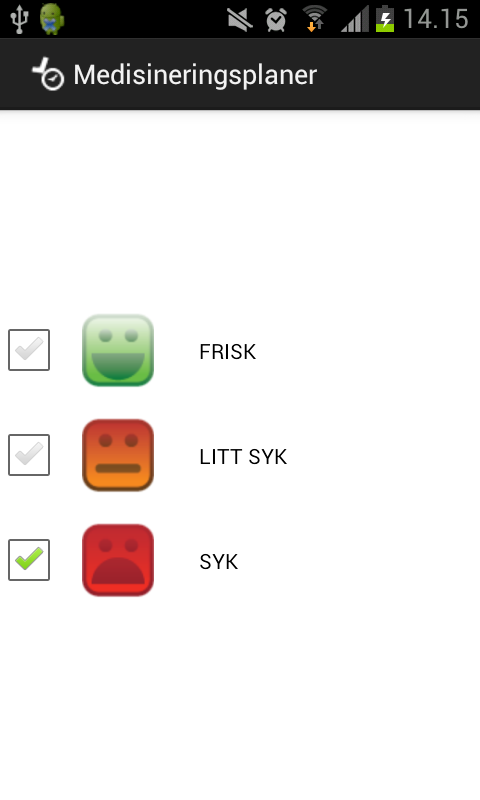
\includegraphics[width=0.20\paperwidth]{Pictures/Screenshots/gapp_view_plans.png}
	\caption{Available plans in GAPP}
	\label{fig:gapp-view-plans}
	\end{minipage}
\end{figure}

\begin{figure}
	\begin{minipage}[b]{0.4\linewidth}
		\centering
		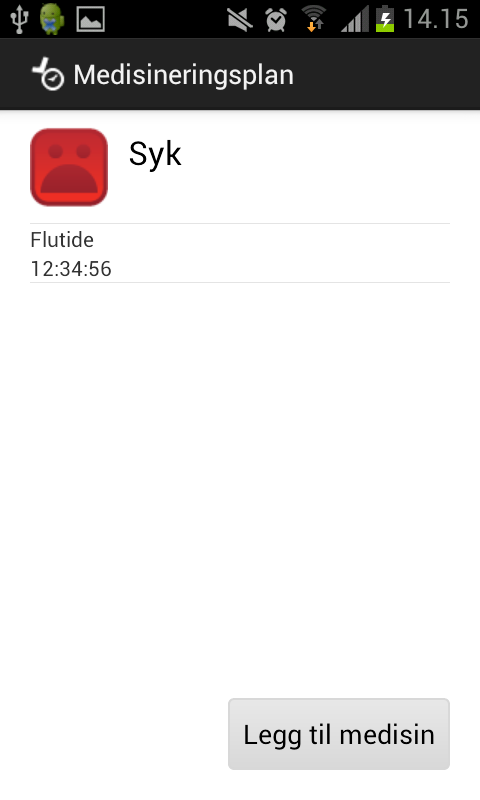
\includegraphics[width=0.20\paperwidth]{Pictures/Screenshots/gapp_plan.png}
	\caption{A medication plan in GAPP}
	\label{fig:gapp-plan}
	\end{minipage}
	\hspace{3cm}
	\begin{minipage}[b]{0.4\linewidth}
		\centering
		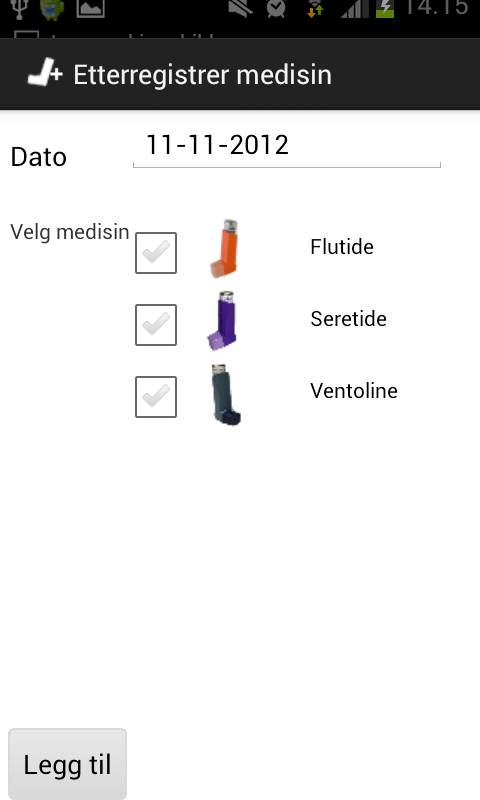
\includegraphics[width=0.20\paperwidth]{Pictures/Screenshots/register_treatment.png}
	\caption{Register treatment in GAPP}
	\label{fig:gapp-register-treatment}
	\end{minipage}
\end{figure}

\begin{figure}
	\begin{minipage}[b]{0.4\linewidth}
		\centering
		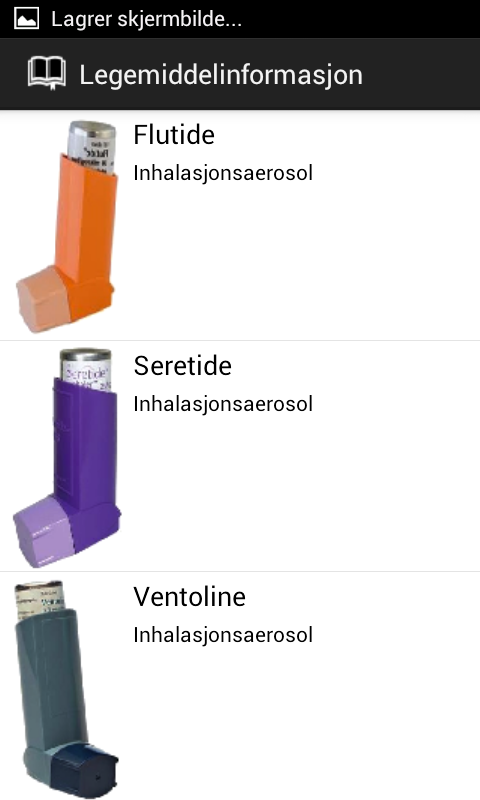
\includegraphics[width=0.20\paperwidth]{Pictures/Screenshots/information.png}
	\caption{Choose among medicines to view more information}
	\label{fig:gapp-infomration}
	\end{minipage}
	\hspace{3cm}
	\begin{minipage}[b]{0.4\linewidth}
		\centering
		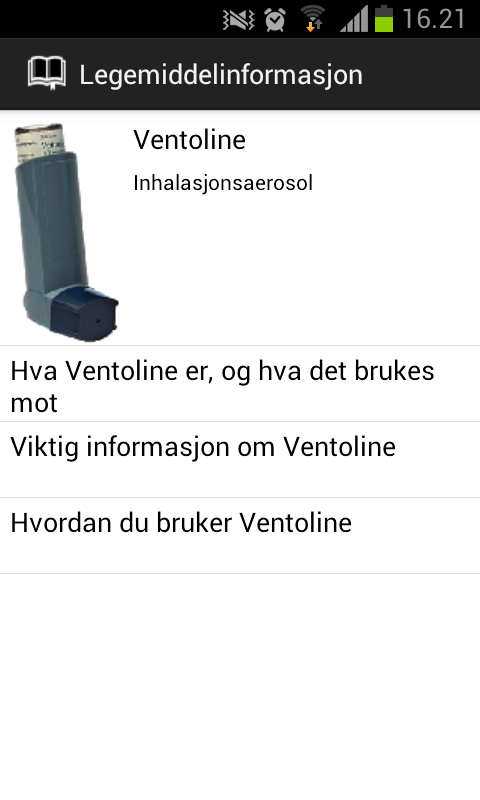
\includegraphics[width=0.20\paperwidth]{Pictures/Screenshots/specific_information.png}
	\caption{Medicine specific information}
	\label{fig:gapp-medicine-information}
	\end{minipage}
\end{figure}


\begin{figure}
	\begin{minipage}[b]{0.4\linewidth}
		\centering
		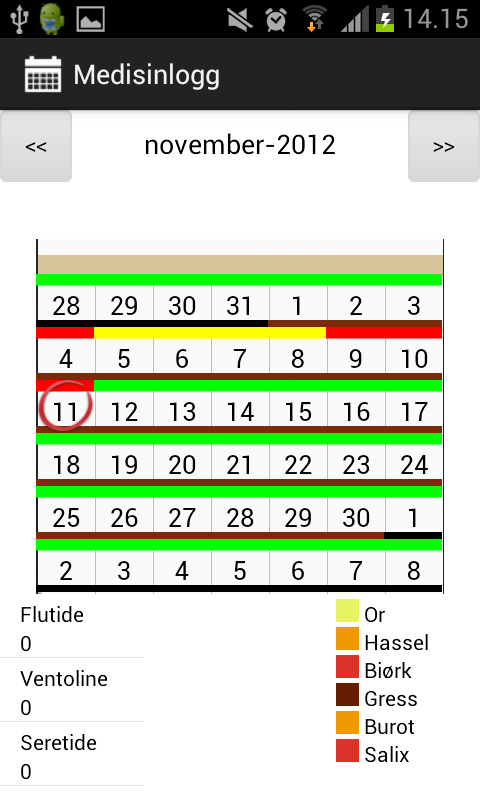
\includegraphics[width=0.20\paperwidth]{Pictures/Screenshots/logg.png}
	\caption{Medicine log in GAPP}
	\label{fig:gapp-log}
	\end{minipage}
\end{figure}




Figure \ref{fig:gapp-main-menu} shows the main menu. The item ``manual'' is a bit misguiding, as this shows an image gallery of 
how a child should take the medicine (shake, put on mask, and so on). We did not have time to make a proper manual on how to use the
application, but hopefully, the application is intuitive enough.


Figure \ref{fig:gapp-view-plans} shows the available plans for an adult. By pressing one of the checkboxes, the child's medical plan
is updated appropriatly. By touching the name of a plan, you get presented with the screen below. 

Figure \ref{fig:gapp-plan} view contains a list of the medicines that are stored in a medicine plan. You can add a medicine through the button, 
and by touching a medicine, you can delete it. 
  

Figure \ref{fig:gapp-log} shows the log of a child.
The log consists mainly of 3 components. The calendar shows the days of a month, the chosen medicine plan for a child on a
given day, indicated by a green/yellow/red line, and the distribution of pollen at that day, indicated by the bottom line of each cell. 


This pollen distribution is given by our dummy xml-feed (since pollenvarslingen.no is not currently casting). 
We have used the same distribution for each day, which explains why every day is brown. Down to the left, one can see how many
times the child has taken the given medicine at a day. Down to the right, you can see the pollen spread at the day for every type 
of pollen that is casted by pollenvarslingen.no. 
The cells of the calendar is touchable, and the listviews on the bottom of the page is updated according to which day is selected.


It is possible to register a treatment after the medication is taken. This is done by choosing the date (which is autofilled with todays date),
and choosing a medicine. The child then gets stars in his/her treasure chest. 

\subsubsection{CAPP - Screenshots}
\label{sec:capp-screenshots}
\begin{figure}
	\begin{minipage}[b]{0.4\linewidth}
		\centering
		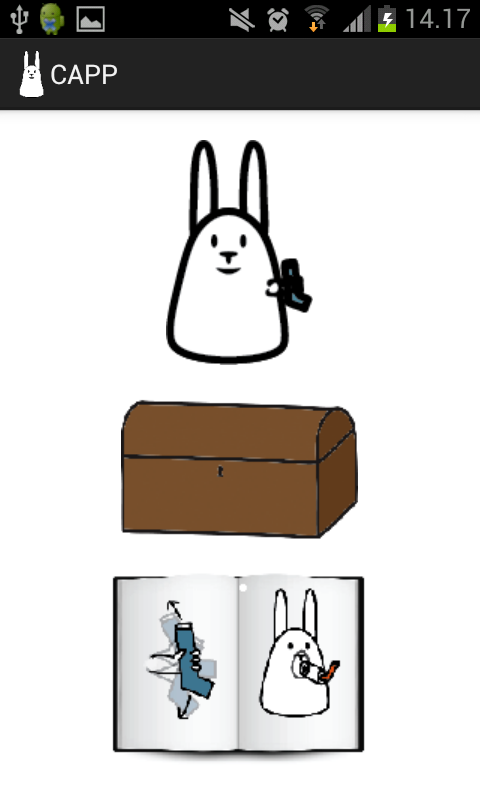
\includegraphics[width=0.20\paperwidth]{Pictures/Screenshots/capp_main_menu.png}
	\caption{Main menu in CAPP}
	\label{fig:capp-main-menu}
	\end{minipage}
	\hspace{3cm}
	\begin{minipage}[b]{0.4\linewidth}
		\centering
		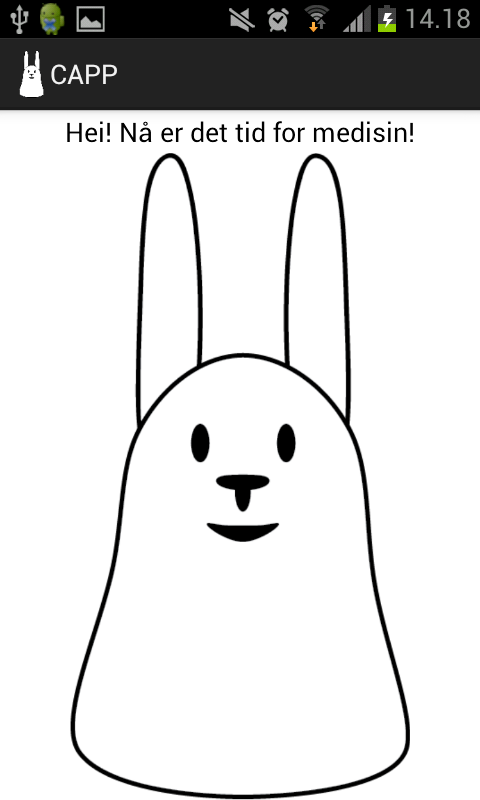
\includegraphics[width=0.20\paperwidth]{Pictures/Screenshots/capp_start_treatment.png}
	\caption{Start a treamtment in CAPP}
	\label{fig:capp-start-treatment}
	\end{minipage}
\end{figure}

\begin{figure}
	\centering
		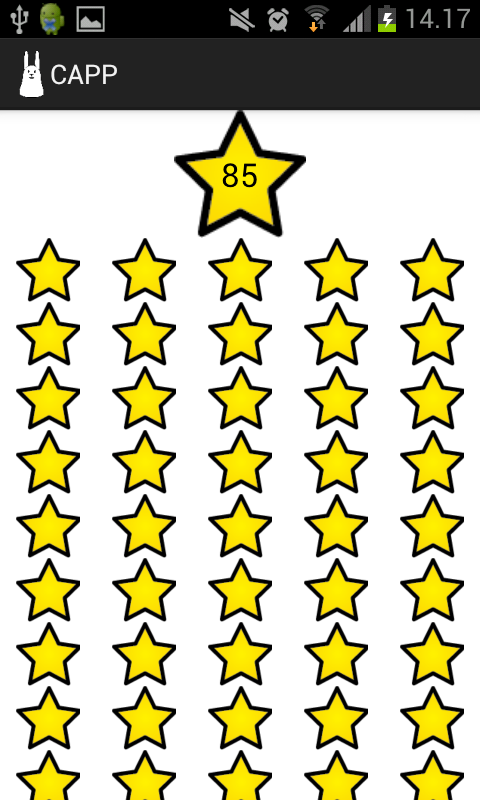
\includegraphics[width=0.20\paperwidth]{Pictures/Screenshots/capp_stars.png}
	\caption{Amount of stars collected in CAPP}
	\label{fig:capp-stars}
\end{figure}

Figure \ref{fig:capp-main-menu} shows the main menu of CAPP. This main menu has three items. To start a treatment, the user chooses the karotz-icon. 
To see amount of stars, the child picks the treasurechest, which leads the user to Figure \ref{fig:capp-stars} 
The book leads to a series of children-friendly images, where the child can have a look at instructions for taking a medicine.   



